\chapter{Validación modelos econométricos}

Se presentan a continuación las validaciones de los modelos econométricos que se ajustaron. Es todos los casos el análisis de residuales fue satisfactorio y no hubo que transformar las variables para corregir algún problema. Para la gráfica de residuales vs ajustados no se observa alguna tendencia y los puntos se ven aleatorios, por este motivo no vemos la existencia de problemas de heterocedasticidad. Además, los residuales siguen una distribución normal por como se ve el QQ-Plot. Por otro lado, en ningún modelo se encontró problemas con datos influyentes o atípicos. 

\newpage

\begin{figure}[H]
\centering
\label{fig:Validacion}
\begin{subfigure}
  \centering
  \caption{Validación modelo AventuraT}
  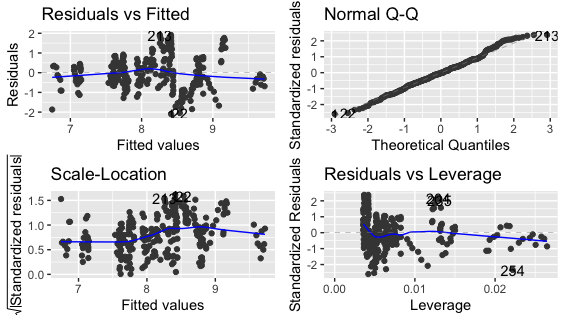
\includegraphics[width=.85\linewidth]{Imagenes/log_avent.png}
\end{subfigure}%
\begin{subfigure}
  \centering
  \caption{Validación modelo Educativo}
  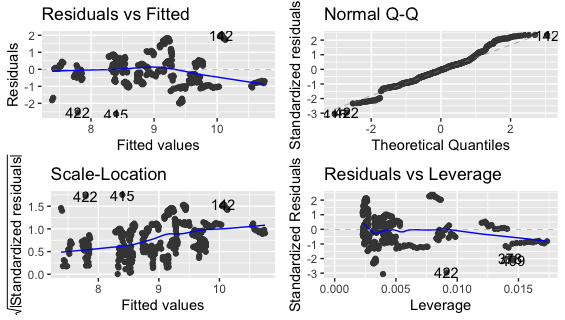
\includegraphics[width=.85\linewidth]{Imagenes/log_educ.png}
\end{subfigure}
\end{figure}

\begin{figure}[H]
\centering
\label{fig:Validacion2}
\begin{subfigure}
  \centering
  \caption{Validación modelo Mi Sueño}
  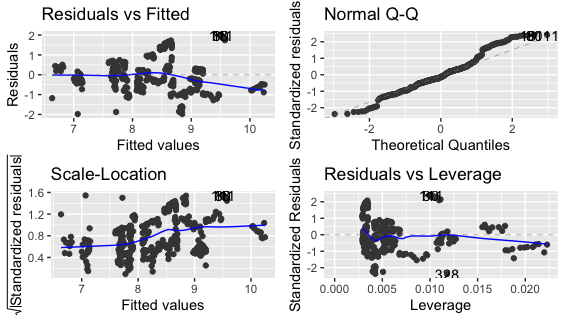
\includegraphics[width=.85\linewidth]{Imagenes/log_suen.png}
\end{subfigure}%
\begin{subfigure}
  \centering
  \caption{Validación modelo Tradicional}
  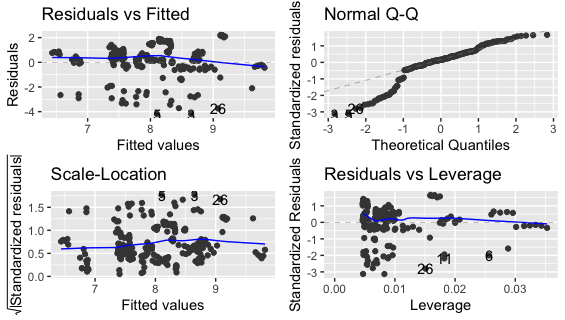
\includegraphics[width=.85\linewidth]{Imagenes/log_trad.png}
\end{subfigure}
\end{figure}

\noindent 